\section{構造体 テンプレート CORBA\_\-Util::has\_\-nil$<$ T $>$}
\label{structCORBA__Util_1_1has__nil}\index{CORBA\_\-Util::has\_\-nil@{CORBA\_\-Util::has\_\-nil}}


has nil traits class template  




{\ttfamily \#include $<$Typename.h$>$}

CORBA\_\-Util::has\_\-nil$<$ T $>$に対する継承グラフ\begin{figure}[H]
\begin{center}
\leavevmode
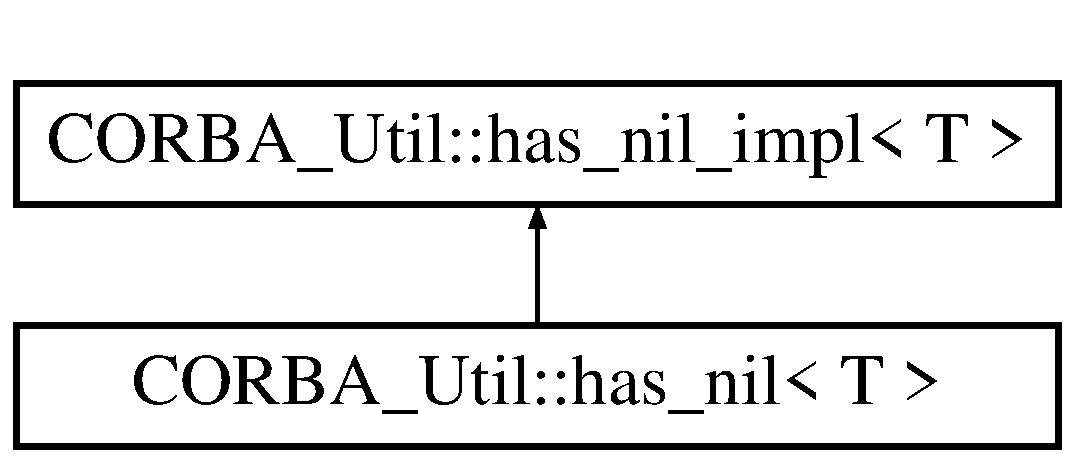
\includegraphics[height=2cm]{structCORBA__Util_1_1has__nil}
\end{center}
\end{figure}


\subsection{説明}
\subsubsection*{template$<$class T$>$ struct CORBA\_\-Util::has\_\-nil$<$ T $>$}

has nil traits class template T has \_\-nil() static function -\/$>$ value = true T has no \_\-nil() static function -\/$>$ value = false 